\documentclass{article}
\usepackage[utf8]{inputenc}
\usepackage{amsmath}

%Import the tikz package
\usepackage{tikz}
\usetikzlibrary{shapes.geometric, arrows}
\usetikzlibrary{positioning}

\title{Assignment 1 - LaTeX and TikZ}
\author{Name}
\date{January 11, 2022}

\begin{document}

\maketitle

%Figure starts here
\begin{figure}[h]
\centering
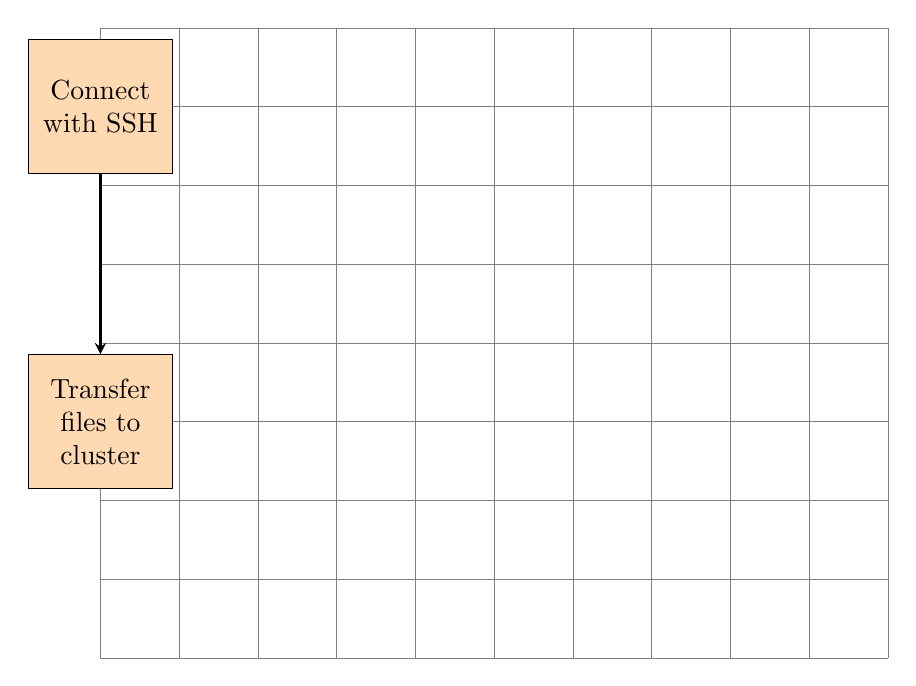
\begin{tikzpicture}

   %Styles of boxes and arrows
   \tikzstyle{processstep} = [rectangle, minimum width=1.7cm, minimum height=1.7cm, text centered, text width=1.6cm, draw=black,  fill=orange!30]
   \tikzstyle{arrow} = [thick,->,>=stealth]
   %--------------------------------------------%
   %          Change styles, if desired         %
   %--------------------------------------------%
   
   %Grid to help with drawing (comment out for final figure)
   \draw[help lines] (0,0) grid (10,8);,
   
   %Boxes 
   \node[processstep] (ssh) at (0,7) {Connect with SSH};
   \node[processstep] (files) at (0,3) {Transfer files to cluster};
   %--------------------------------------------%
   %            Add remaining boxes             %
   %--------------------------------------------%
   
   %Arrows
   \draw[arrow] (ssh.south) -- (files.north);
   %--------------------------------------------%
   %           Add remaining arrows             %
   %--------------------------------------------%
  

\end{tikzpicture} 
\end{figure} 

\end{document}
